%% -*- mode: latex; mode: flyspell -*-
\documentclass[12pt, letter]{article}

%% Class name and Assignment number
%%
\newcommand{\courseName}{CSC421: Artificial Intelligence}
\newcommand{\assignName}{Assignment~2}

%% Packages
\usepackage{amsmath,amsfonts,amssymb,amsthm,dsfont}
\usepackage{physics}
\usepackage{graphicx}
\usepackage[bookmarks=false]{hyperref}
\usepackage{color}
\usepackage{lipsum}
\usepackage{placeins}
\usepackage{float}
\restylefloat{table}

%% Paper format
\usepackage{geometry}
\geometry{
    letterpaper,
    %% total={216mm,279mm}, %< NSERC size
    margin=2.00cm,     %< default
    %% margin=1.87cm,       %< NSERC tightest
}

%% Headers and footers
\usepackage[explicit]{titlesec}
\newpagestyle{titlesec_assignment}{
  \sethead{\courseName}{}{\assignName}\setfoot{}{\thepage}{}
  \headrule
  %% \footrule
}

\begin{document}

%% Set header and footer
\pagestyle{titlesec_assignment}

%% Title
\title{\courseName\\\assignName}
\author{Rafael Solorzano}
\maketitle

\section{Introduction}

 In this assignment Probabilist Simulation is explored by simulating two different monopoly games. In the first one, only landings on spots and chance cards occurrences are recorded, whereas the second one includes more rules to handle money and decide a winner between two player over 50 turns each. This is presented in Section 2. 

The Naive Bayes learning is done with a set of positive and negative reviews that take into account only a binary Vector of words, in order to get probabilities. The predictions is done both with a 10-fold version and a simple version. This is presented in Section 3. 

\section{Monopoly}

\subsection{Dice Generation}

The dice generation for the Monopoly game is done by using the randint from python. It will generate the rolling of two numbers between 1 and 6 that will represent the two dice. The code for the dice generation is shown in Figure 1. The code to handle doubles is done during the Monopoly game simulation, the dice generation just simulates the rolling of two dice. 

 \begin{figure}[htb]
  \centering
  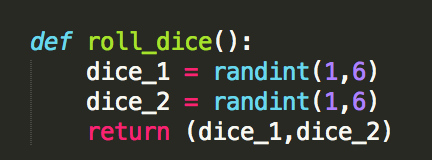
\includegraphics[width=0.40 \textwidth]{./figures/dice.png}
  \caption{The Dice Generator.}
\end{figure}

\subsection{Chance Cards}

Chance cards are simulated in the game, with most of them implemented in either the Probability or Multiplayer version of the game. The Get Out of Jail Free and Pay Repair cards are the only cards that are not implemented.

The chance cards are held in a dictionary that represent all the 16 cards in the game. This dictionary contains the name, and the number of times each chance card has been pulled. They are placed in order in a "Deck" and the shuffled at the beginning of the simulation. Once a call is pulled it is placed back at the end of the deck. The code that handles getting a chance card is shown in Figures 2, 3, and 4 below. 

 \begin{figure}[htb]
  \centering
  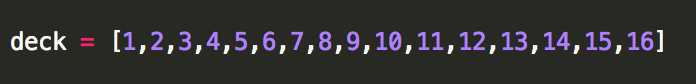
\includegraphics[width=0.50 \textwidth]{./figures/deck.png}
  \caption{Shuffle the global deck, only called once.}
\end{figure}

 \begin{figure}[htb]
  \centering
  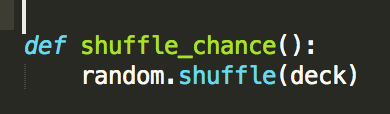
\includegraphics[width=0.40 \textwidth]{./figures/shuffler.png}
  \caption{Shuffle the global deck, only called once.}
\end{figure}

 \begin{figure}[htb]
  \centering
  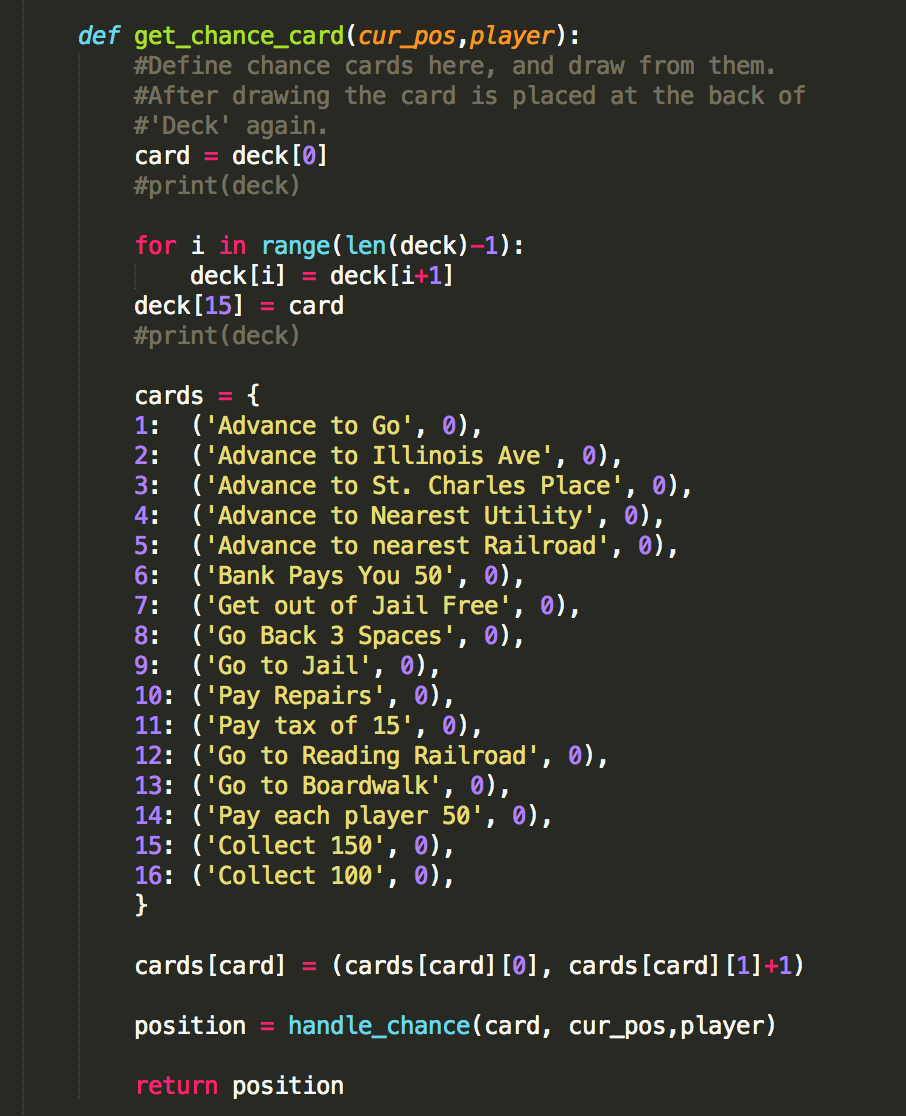
\includegraphics[width=0.75 \textwidth]{./figures/get_chance.png}
  \caption{The get chance card function.}
\end{figure}

\FloatBarrier

Aside from the get chance card function, a handle chance function is used in order to handle the card that was pulled. It will return a position to move to if the card yielded a result that requires movement or 0 otherwise. A sample code from the non-multiplayer version is shown in Figure 5 below, the changes for the multiplayer version will be shown in that section.

 \begin{figure}[htb]
  \centering
  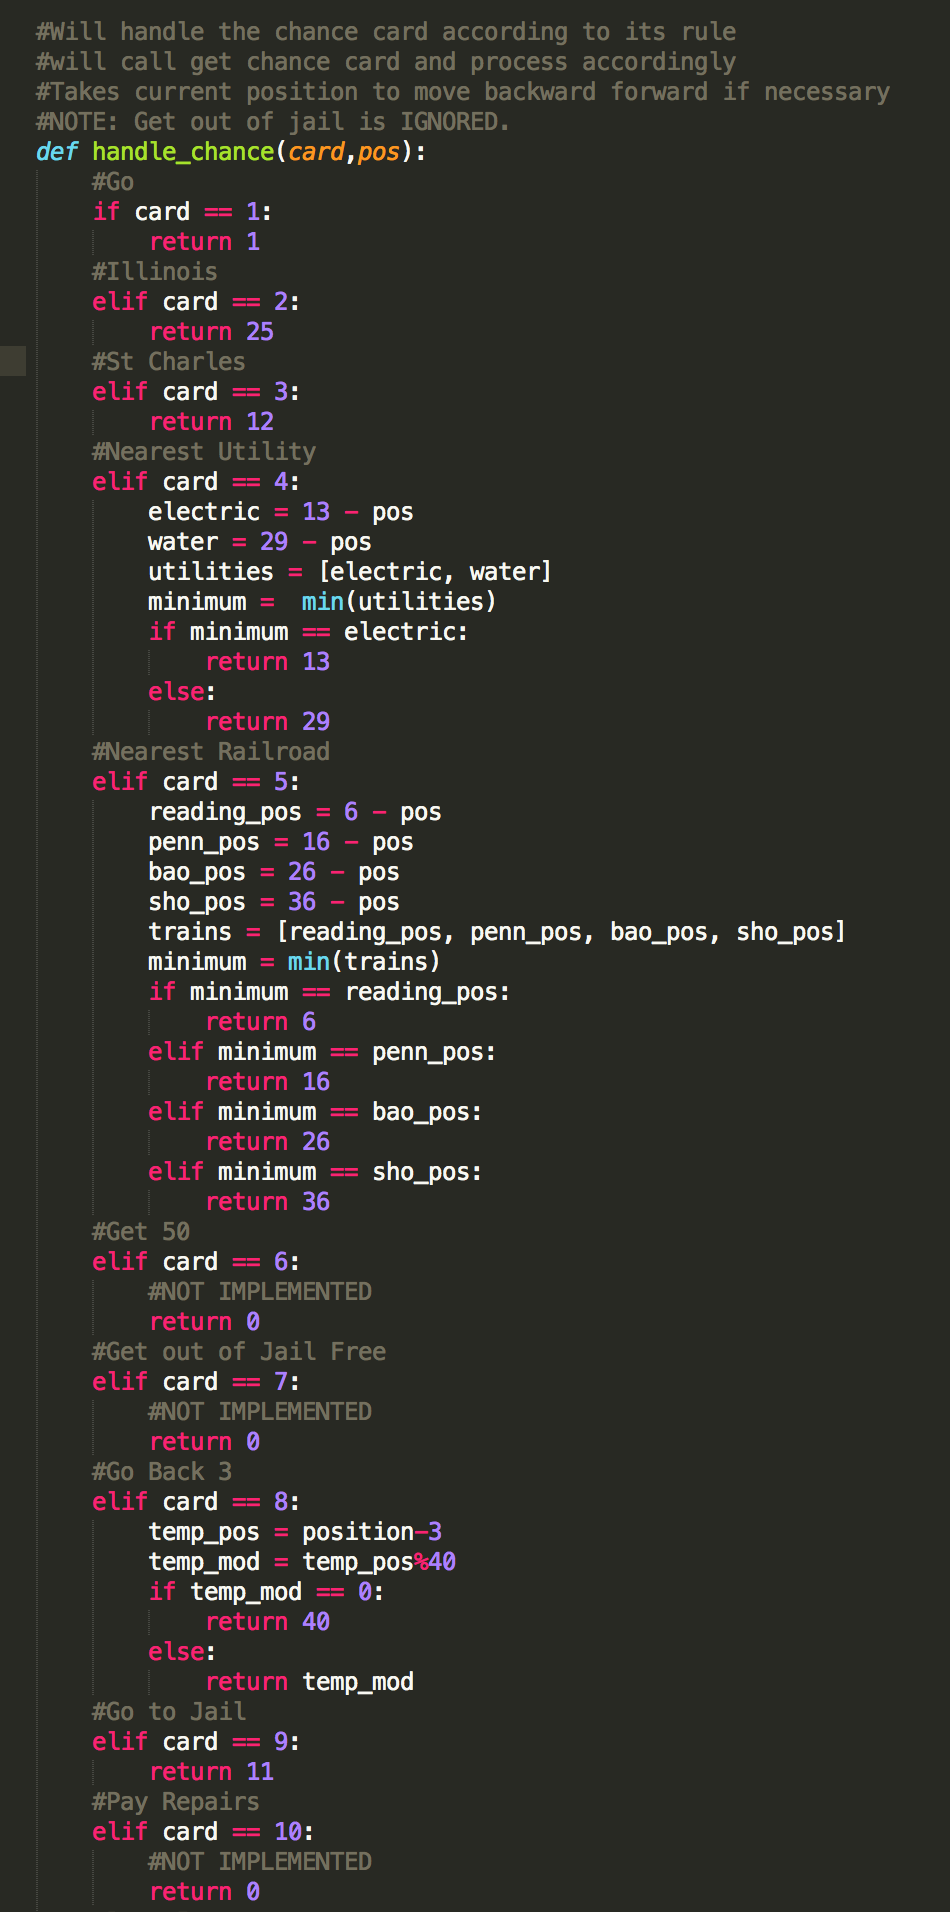
\includegraphics[width=0.6 \textwidth]{./figures/handle_chance.png}
  \caption{The handle chance card function.}
\end{figure}

\FloatBarrier

\subsection{Game Simulation and Probabilities}

The probabilities game simulation consists of a play monopoly function. This function contains a dictionary similar to the chance dictionary that contains the landing for each property as well as the name of each space. The Initial shuffle and board dictionary is shown in Figure 6.

The main game logic is contained in a for loop that will keep rolling the dice and counting the spaces landed on, a check for the doubles is done here. Note that for double calculation the player will not be sent to jail after three consecutive doubles, instead the player will keep rolling until they no longer get doubles. The code for the main game logic is shown in Figure 7 below. 

Finally, the code that will run the monopoly game 1000 times and get the probabilities is shown in Figure 8 below. The code will run 1000 independent games of monopoly and will keep the probability of all the railroads, the GO square, Mediterranean Avenue, and Boardwalk as required by the assignment. The summary of these landings is presented in Table 1. 

 \begin{figure}[htb]
  \centering
  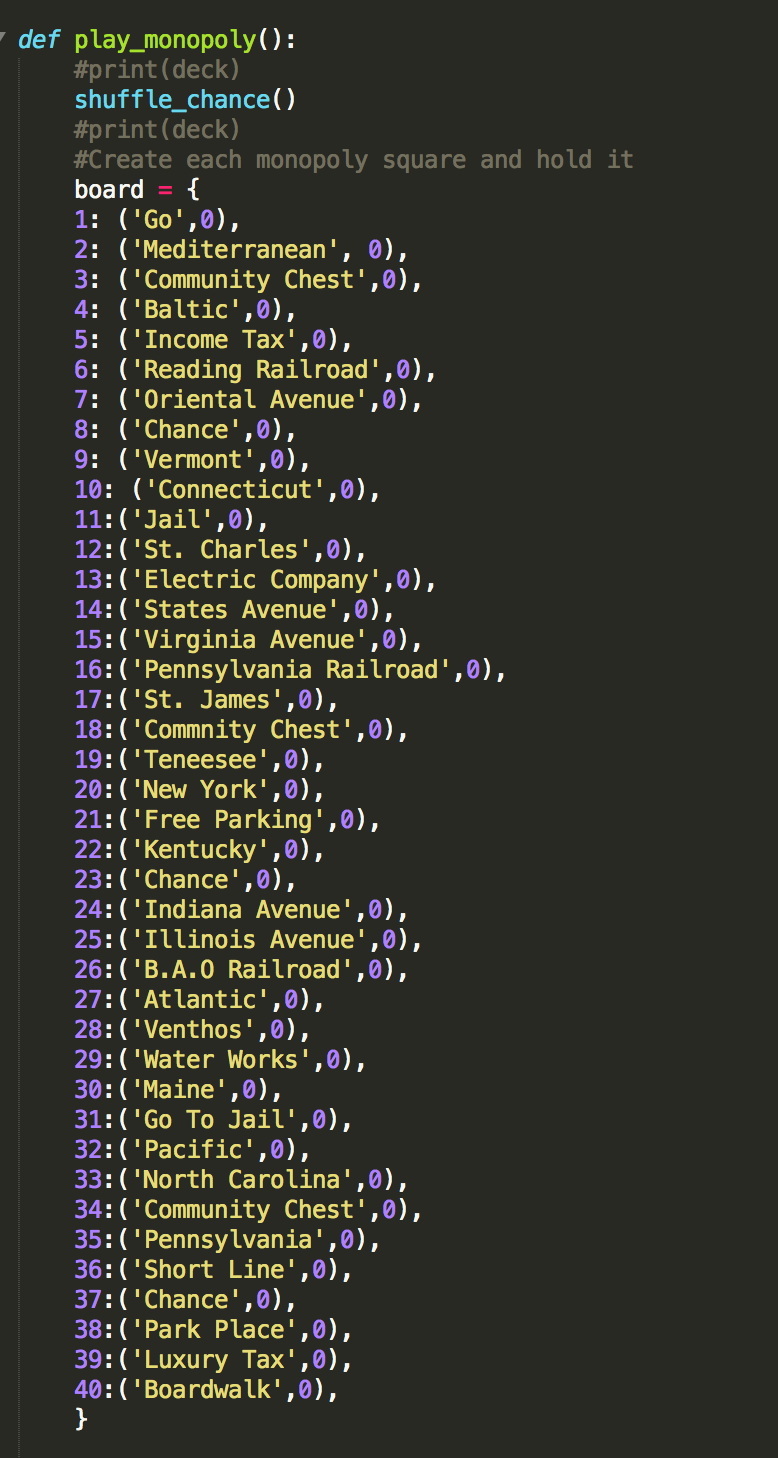
\includegraphics[width=0.6 \textwidth]{./figures/monopoly_board.png}
  \caption{The initial Monopoly function.}
\end{figure}

 \begin{figure}[htb]
  \centering
  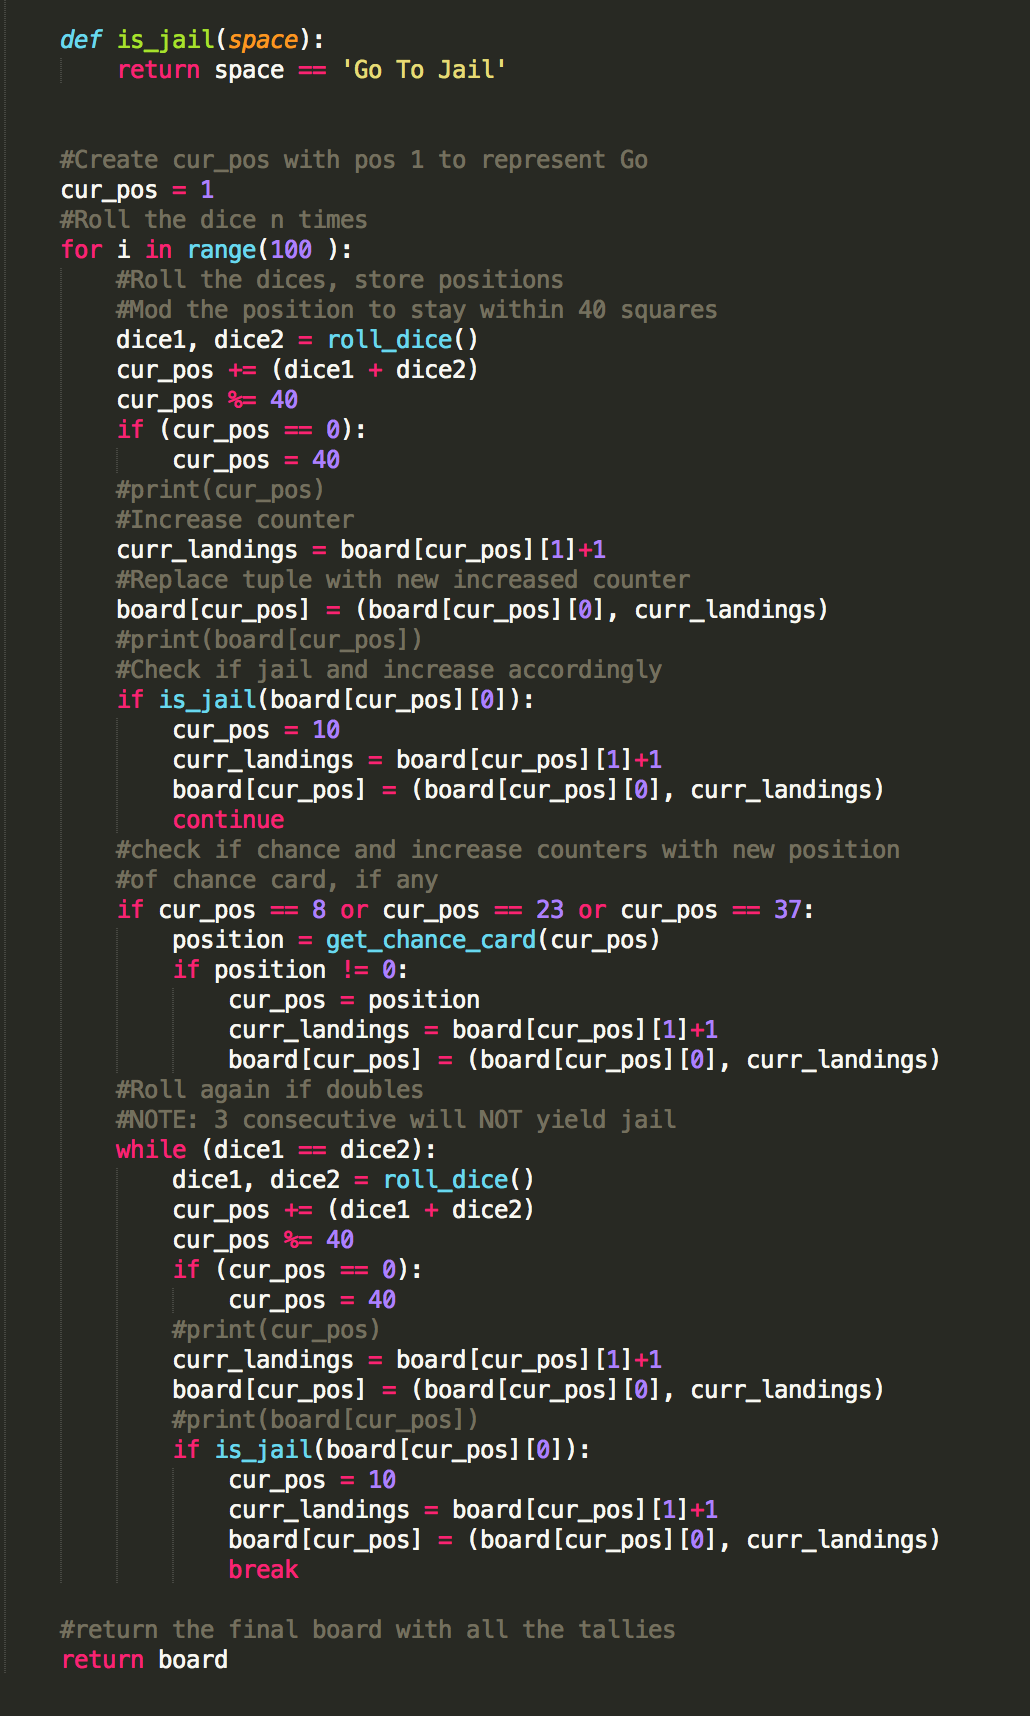
\includegraphics[width=0.7 \textwidth]{./figures/monopoly_loop.png}
  \caption{The main Monopoly loop.}
\end{figure}

 \begin{figure}[htb]
  \centering
  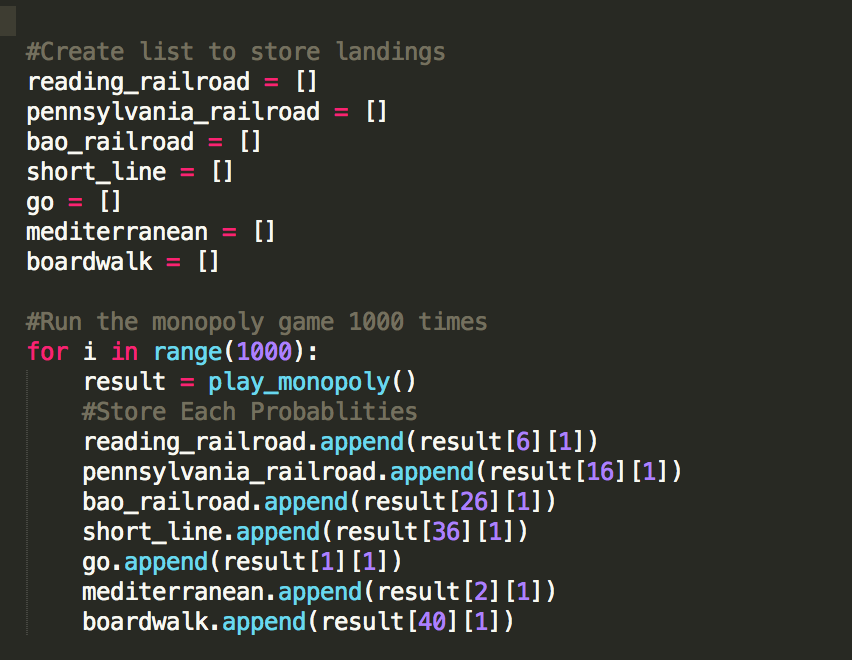
\includegraphics[width=0.7 \textwidth]{./figures/monopoly_probs.png}
  \caption{The 1000 game Monopoly loop.}
\end{figure}

\begin{table}[]
\centering
\caption{Probabilities of landing in selected spaces. }
\label{my-label}
\begin{tabular}{llll}
 & Space                 & Total Landings & Probability of Landing \\
 & Reading Railroad      & 3651           & 3.65\%                 \\
 & Pennsylvania Railroad & 3224           & 3.22\%                 \\
 & BAO Railroad          & 3196           & 3.19\%                 \\
 & Short Line            & 2812           & 2.81\%                 \\
 & Go                    & 3015           & 3.01\%                 \\
 & Mediterranean Ave     & 2576           & 2.57\%                 \\
 & Boardwalk             & 2980           & 2.98\%                
\end{tabular}
\end{table}

\FloatBarrier

\subsection{Multiplayer Game Simulation}

The multiplayer game simulation includes the addition of money to the game, and only accounts for a 2 player game. A main difference from the single player version is in the board, as it now includes an owner,  cost of buy and rent. The code of the modified board dictionary is shown in Figure 9. 

The simulation accounts for buying properties, this is done by a landing property function, which will semi randomly decide if a player will buy the property of not. It was decided to add a rich flag to add a little bit more realism to the game, this will make the player always buy a property as long as it has over 400 in money. After the player is below this, buying will be decided with a random generation of 1 and 2, 1 representing buy and 2 representing not buy. The code for this function is shown in Figure 10.

The two tax properties are handled in the game as well, initially they are detected by the land on property function and handled by the check tax function, in which the corresponding amount will be deducted from the player. The code of the tax function is shown in Figure 11. 

Paying of rent in a simplified way is handled by the game as well, this is done by using the fixed rent price of each property. Multiple colours, house, or hotels are not accounted for. Additionally, multiple railroads or the way landing in a an utility payments are done is not handled instead they each have a fixed rent. The code to handle rent in shown in Figure 12. 

A give go function was also added to the game that will give the players 200 when they pass go. This function is called on the main monopoly loop. The give go function is shown in Figure 13. Additionally, some extra functionality that either adds or subtracts money from a player given a chance cards was added, a sample of the code is shown in Figure 14. This code is a modified version of the code shown in Figure 5, it includes more implementations that deal with money.  

The main Monopoly loop was modified to account for changed of handling landings, go, ending the game of bankruptcy, and changing the output. The main additions are shown in Figure 15 and 16. Finally, a sample output of the initial game is shown in Figure 17, note that Chance cards results are not printed.

 \begin{figure}[htb]
  \centering
  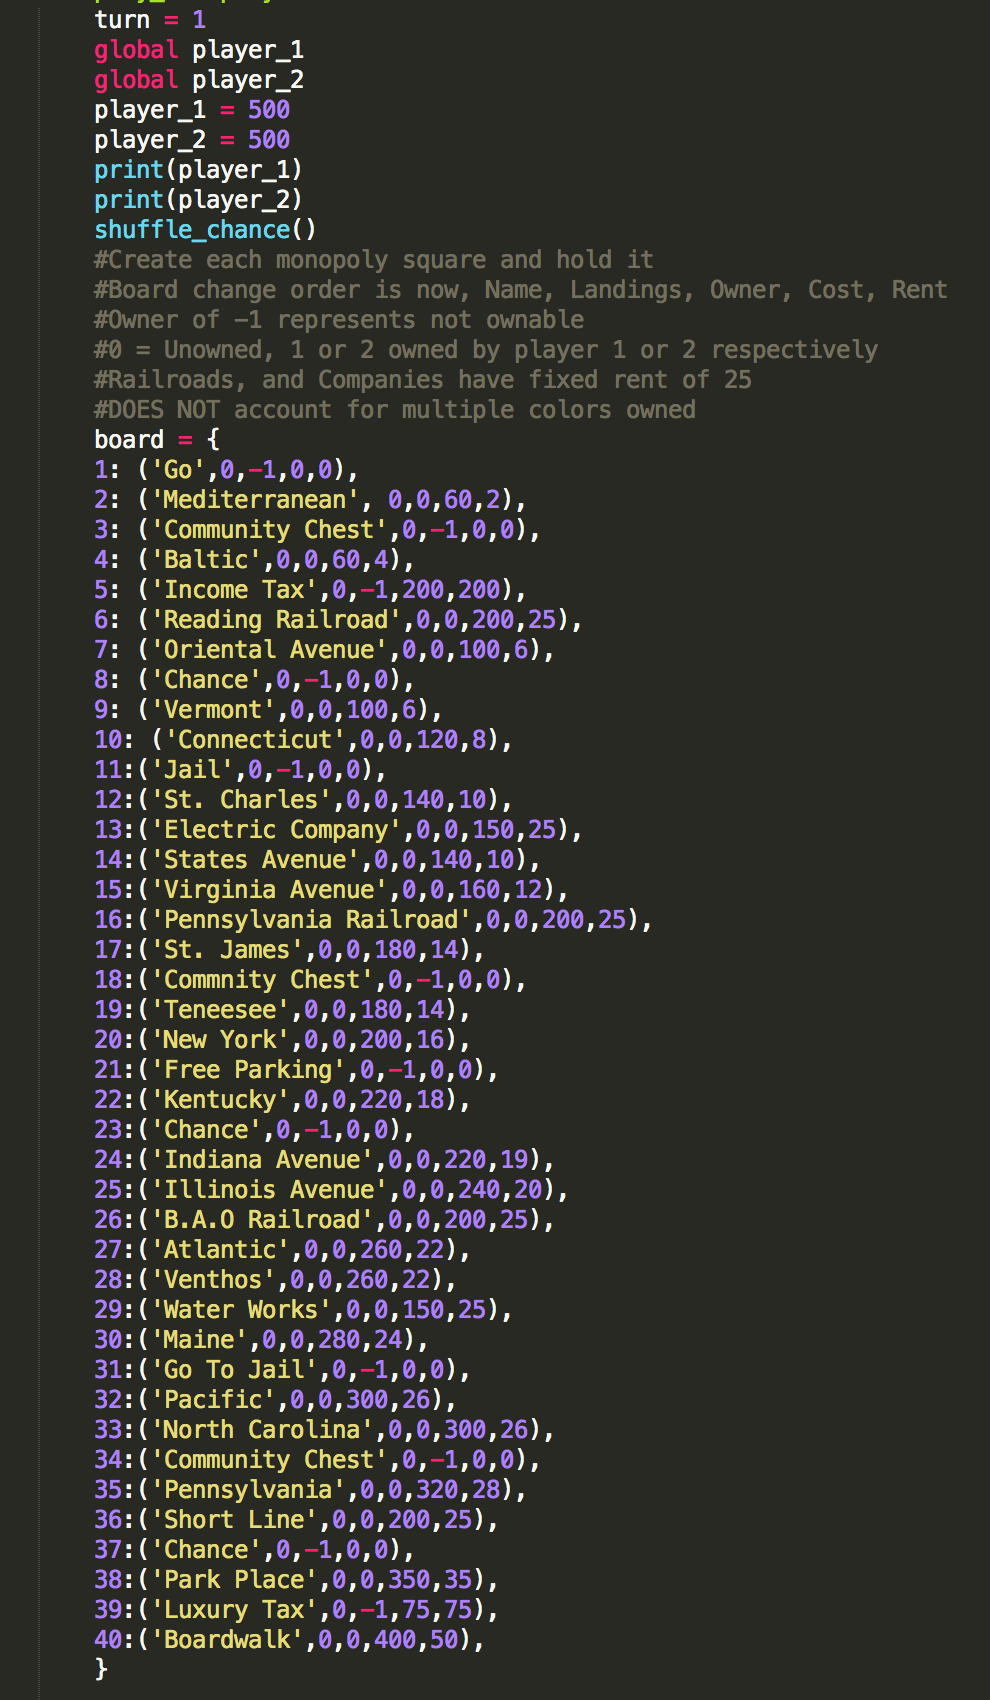
\includegraphics[width=0.7 \textwidth]{./figures/board_multiplayer.png}
  \caption{The Multiplayer board.}
\end{figure}

 \begin{figure}[htb]
  \centering
  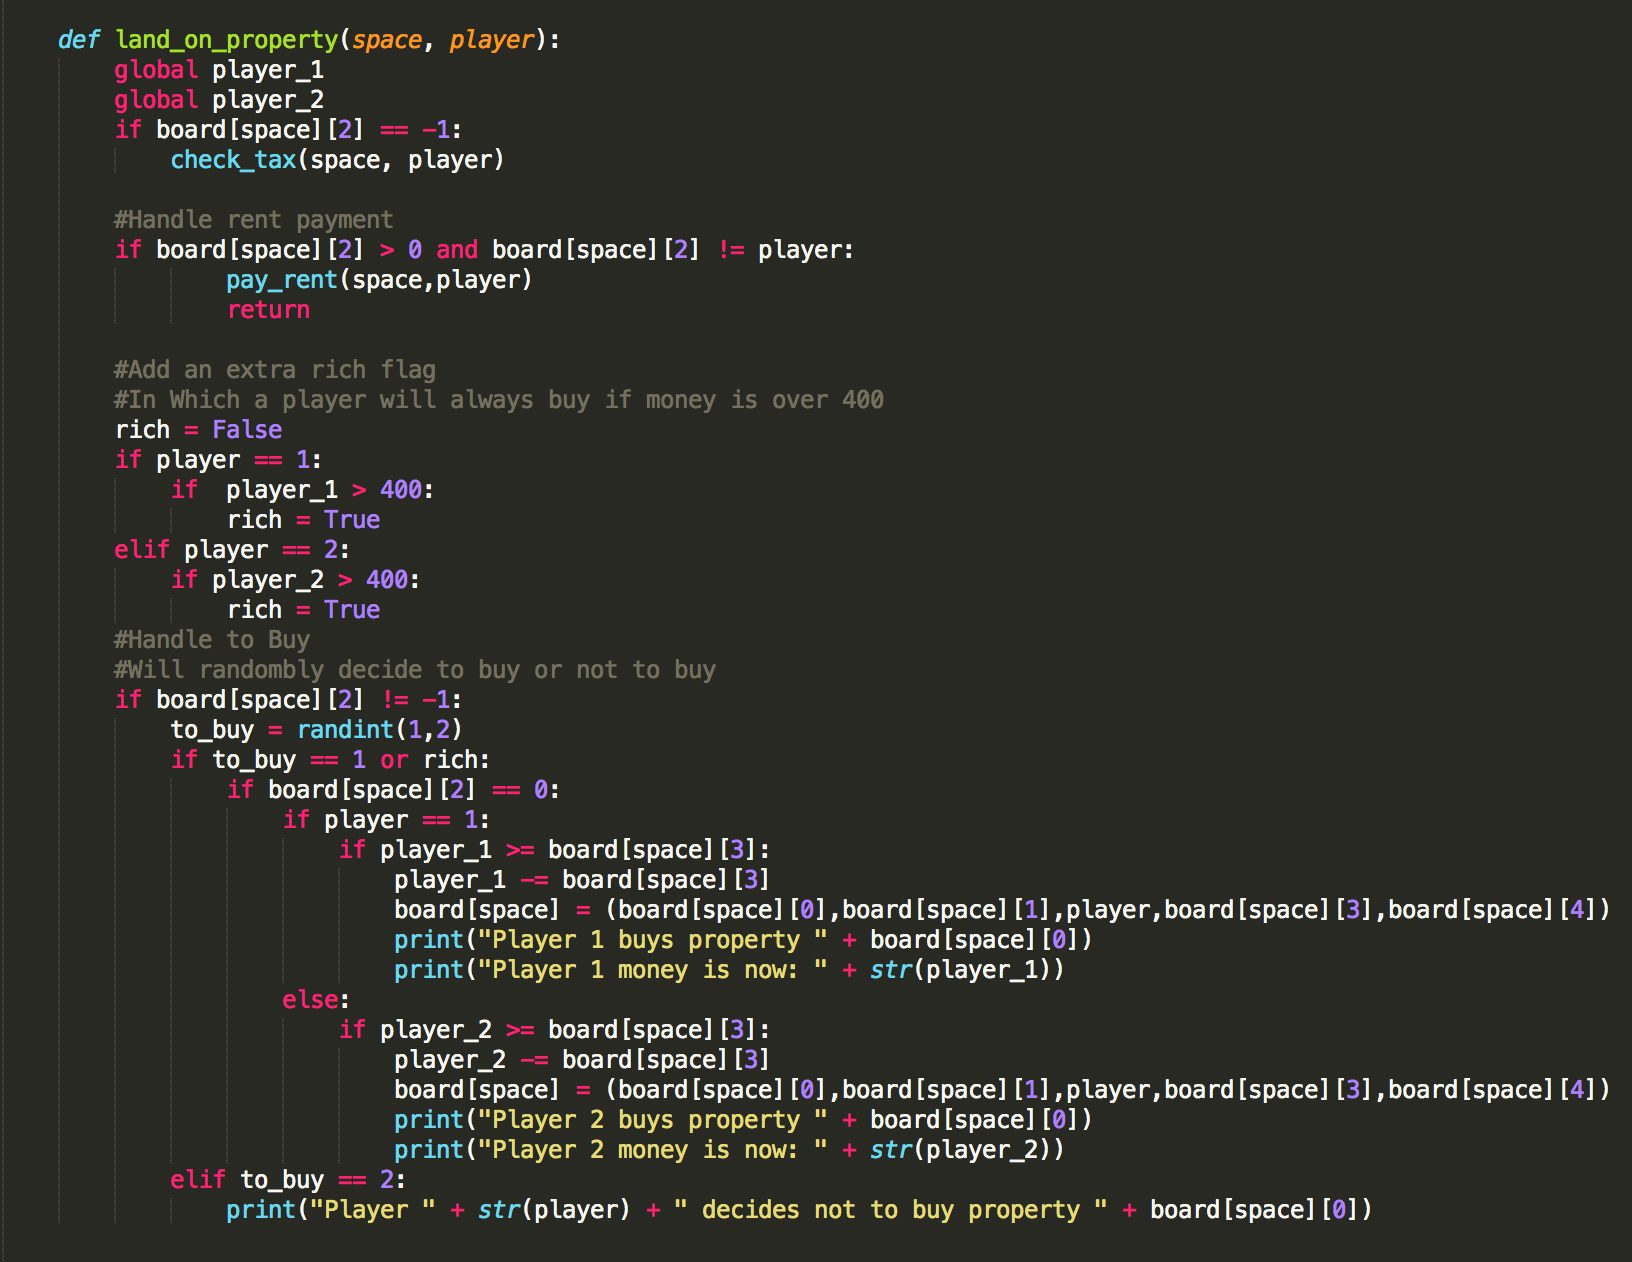
\includegraphics[width=0.9 \textwidth]{./figures/land_on.png}
  \caption{The land on property handler.}
\end{figure}

 \begin{figure}[htb]
  \centering
  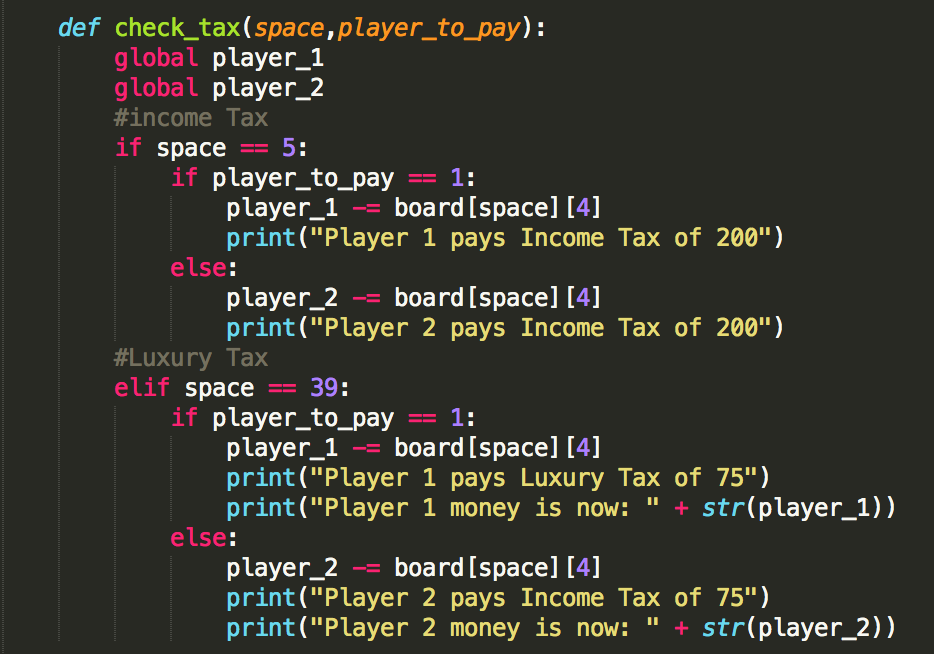
\includegraphics[width=0.7 \textwidth]{./figures/tax.png}
  \caption{The tax function.}
\end{figure}

 \begin{figure}[htb]
  \centering
  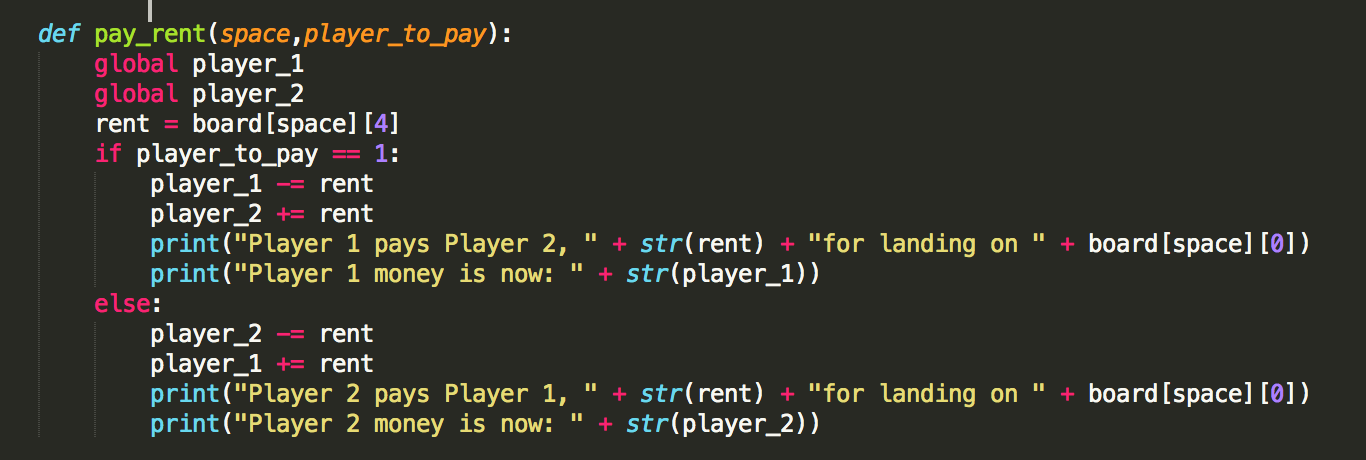
\includegraphics[width=0.8 \textwidth]{./figures/rent.png}
  \caption{The rent function.}
\end{figure}

 \begin{figure}[htb]
  \centering
  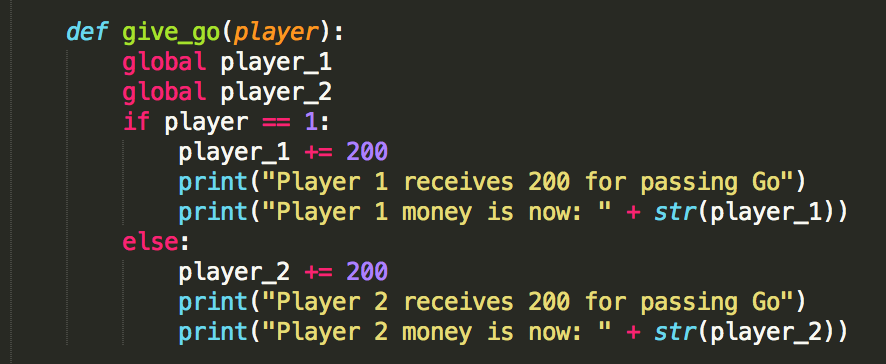
\includegraphics[width=0.7 \textwidth]{./figures/give_go.png}
  \caption{The GO function.}
\end{figure}

 \begin{figure}[htb]
  \centering
  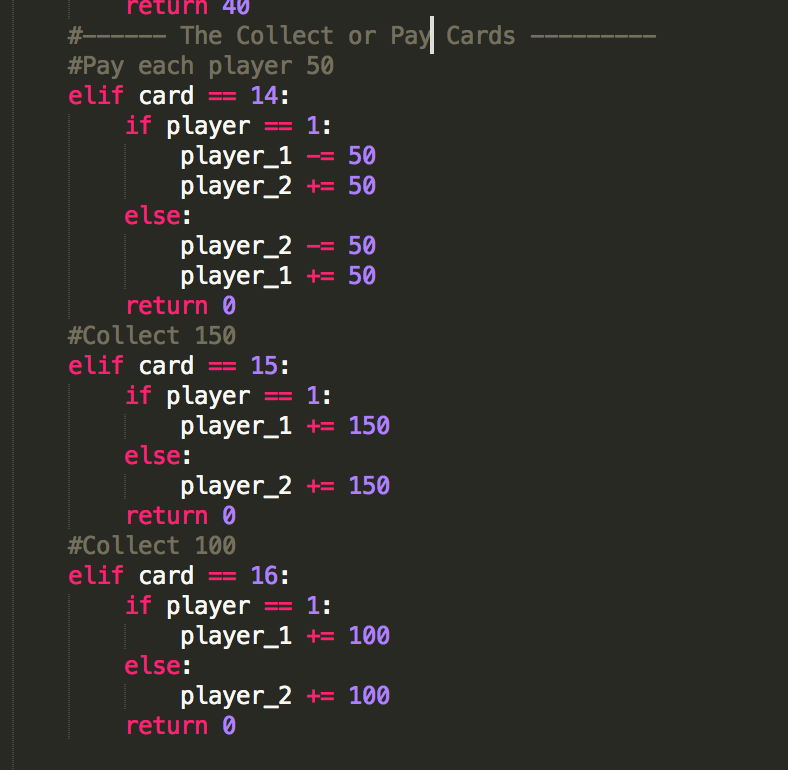
\includegraphics[width=0.7 \textwidth]{./figures/extra_chance.png}
  \caption{The Collect and Pay Implementations.}
\end{figure}

 \begin{figure}[htb]
  \centering
  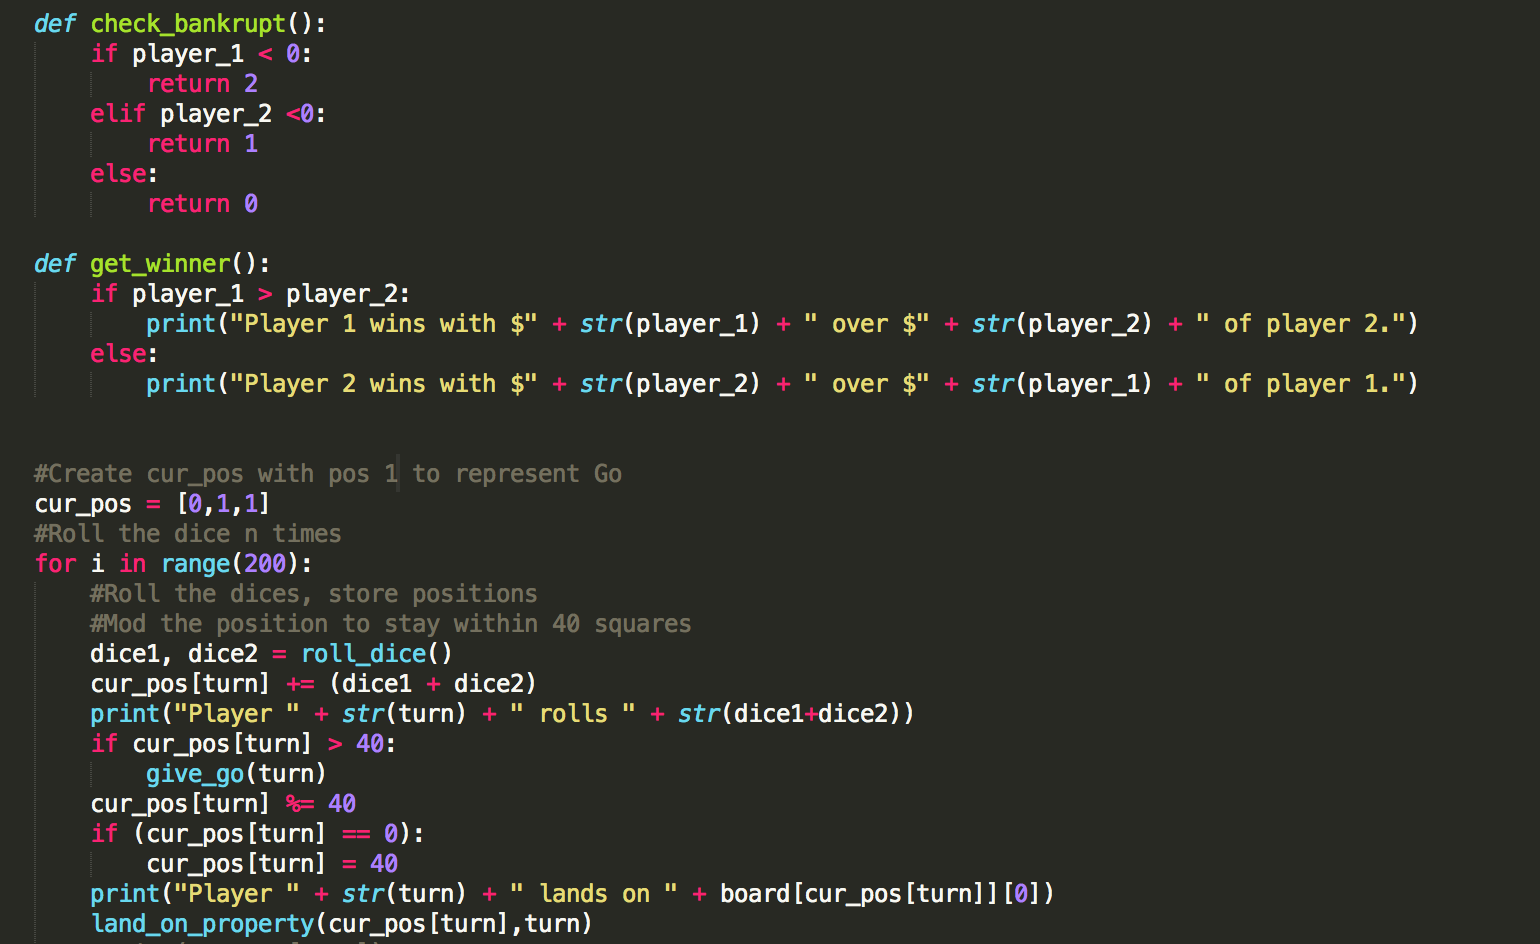
\includegraphics[width=0.9 \textwidth]{./figures/multi_one.png}
  \caption{Additions of main monopoly loop.}
\end{figure}

 \begin{figure}[htb]
  \centering
  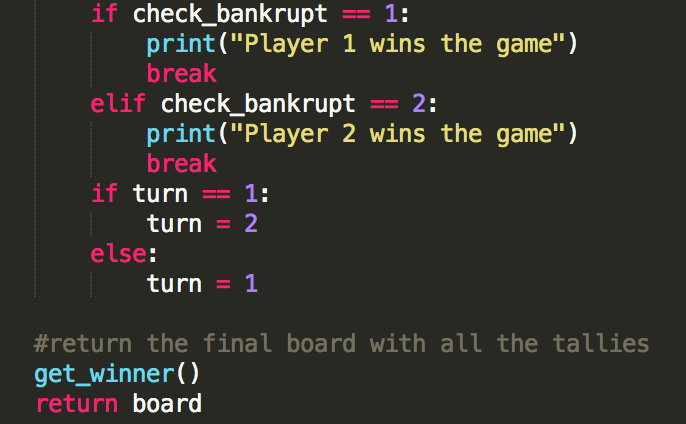
\includegraphics[width=0.7 \textwidth]{./figures/multi_2.png}
  \caption{The end game additions.}
\end{figure}

 \begin{figure}[htb]
  \centering
  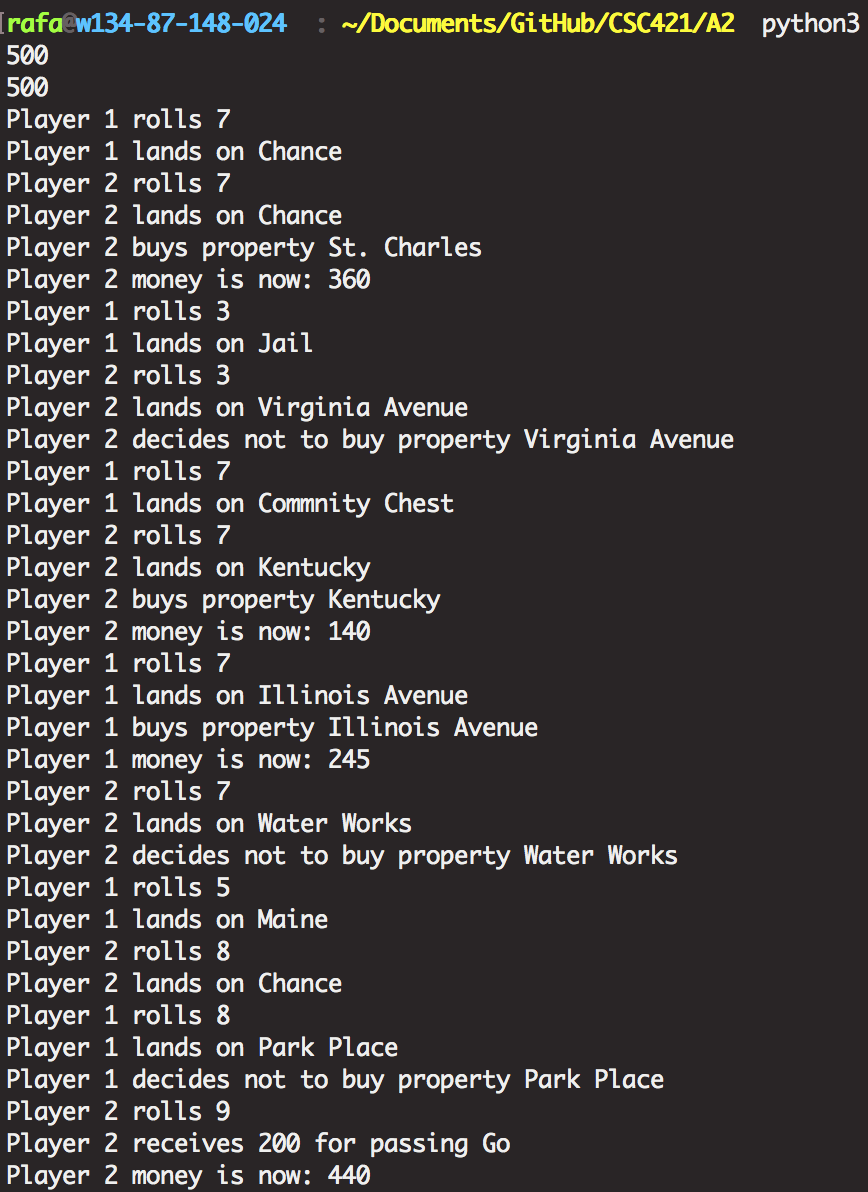
\includegraphics[width=0.7 \textwidth]{./figures/sample_multi.png}
  \caption{The sample output of two player Monopoly.}
\end{figure}

\FloatBarrier


\section{Naive Bayes}

\subsection{Word Probabilities}

The code that parses the text files and stores them in Vector representation is shown in Figure 18. Note that only the code for the positive reviews is shown, the negative reviews is exactly the same with the only difference of reading txt files from the neg folder. 

The probabilities for each dictionary word in the positive and negative reviews are calculated by the code shown in Figure 19. Further, the result of this calculations is shown in Figure 20. 


 \begin{figure}[htb]
  \centering
  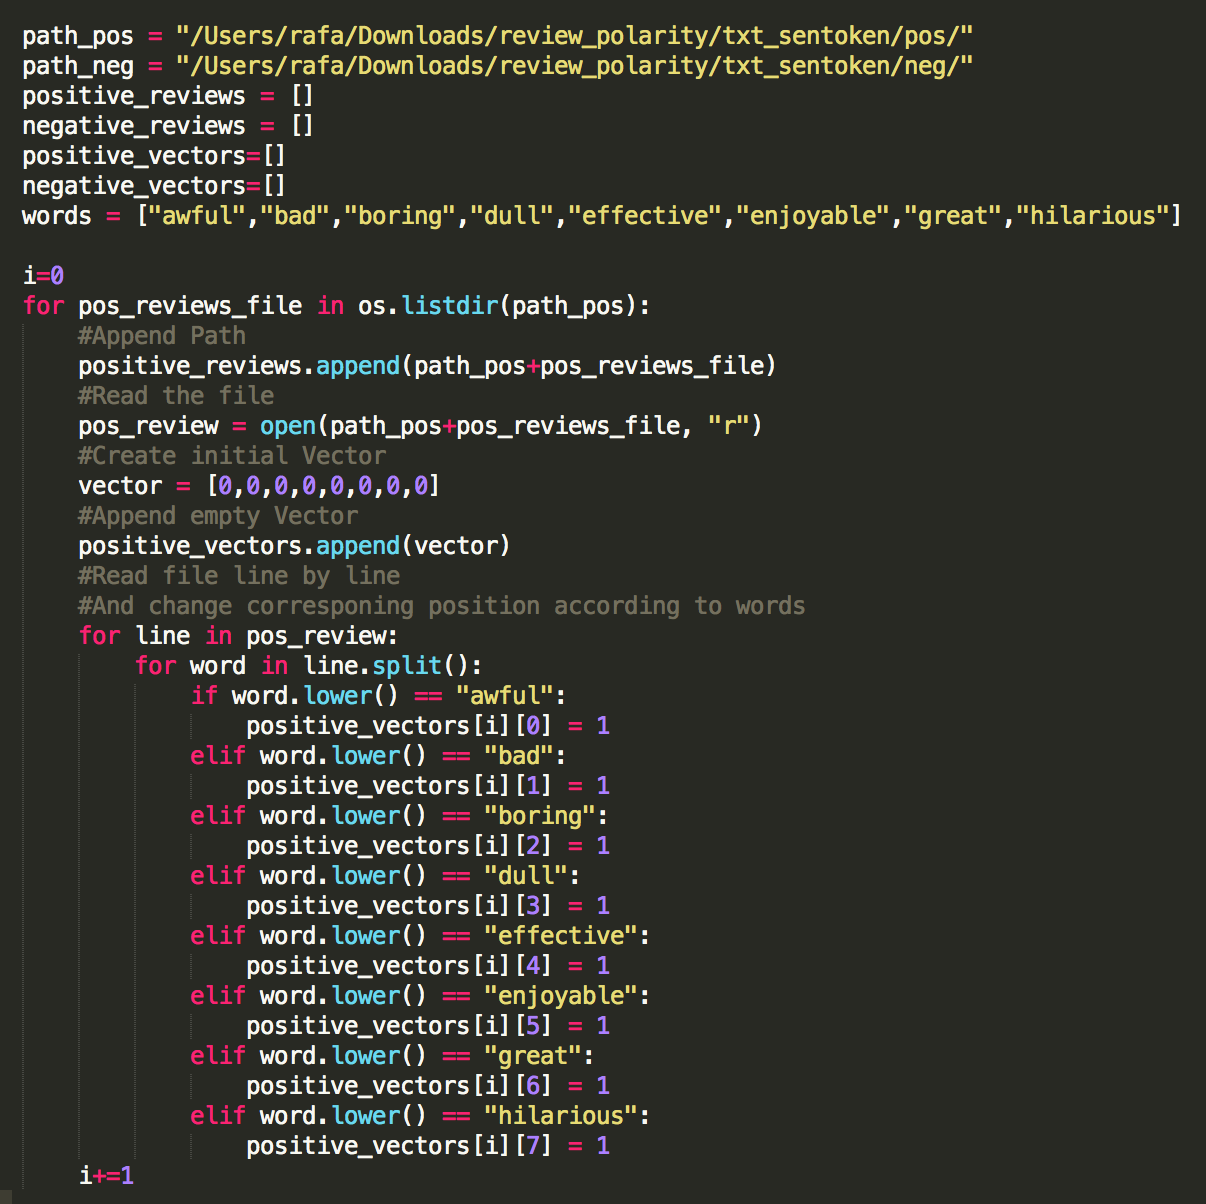
\includegraphics[width=0.7 \textwidth]{./figures/parsing.png}
  \caption{Parsing the txt files.}
\end{figure}

 \begin{figure}[htb]
  \centering
  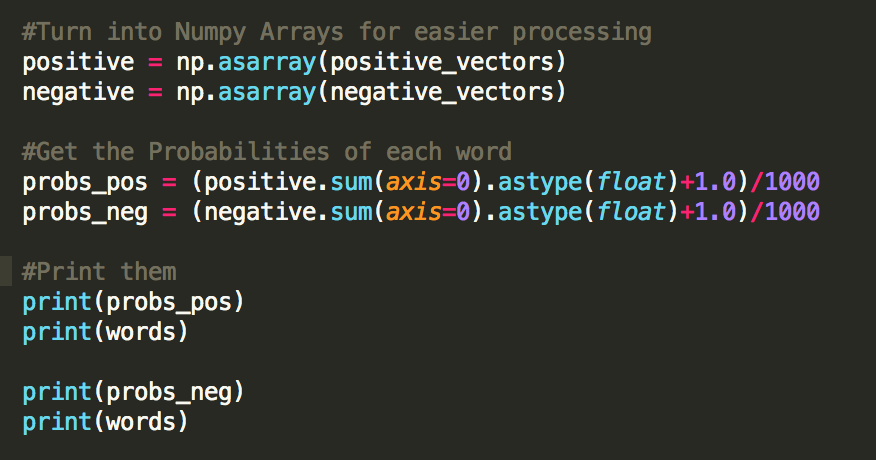
\includegraphics[width=0.7 \textwidth]{./figures/probs.png}
  \caption{Calculating the probabilities for each word.}
\end{figure}

 \begin{figure}[htb]
  \centering
  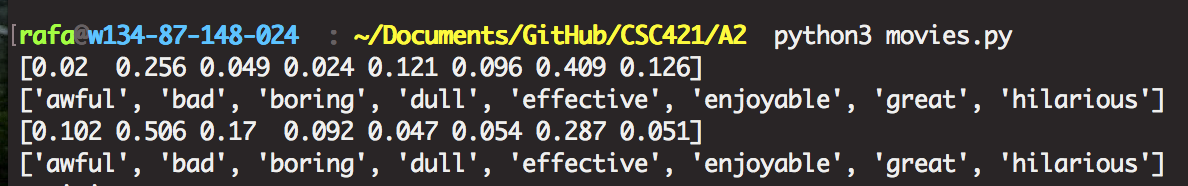
\includegraphics[width=0.7 \textwidth]{./figures/probs_print.png}
  \caption{The result of the probabilities.}
\end{figure}

\FloatBarrier

\subsection{Naive Bayes Classifier}

The probabilities estimates can be combined to form a Naive Bayes classifier in the sense that they are a binary representation, therefore we don't care on the total number of occurrences of each word but instead on the sole occurrence of each word. We calculate the likelihood of each word using a simplified Bayes in which we only use probability of the word appearing. This is done in the likelihood function shown in Figure 21. 

 \begin{figure}[htb]
  \centering
  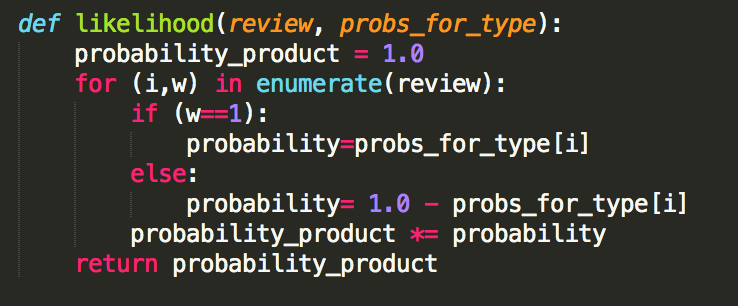
\includegraphics[width=0.7 \textwidth]{./figures/likelihood.png}
  \caption{The likelihood calculation, using Naive Bayes.}
\end{figure}

\FloatBarrier

\subsection{Classification Accuracy and Confusion Matrix}

The confusion matrix for this problem is shown in Table 2. Further, the code to calculate the classification accuracy for this problem is shown in Figure 22. The results obtained by these code are a classification accuracy of 75.6\% for the positive review set and 59.2\% for the negative reviews set.

 \begin{figure}[htb]
  \centering
  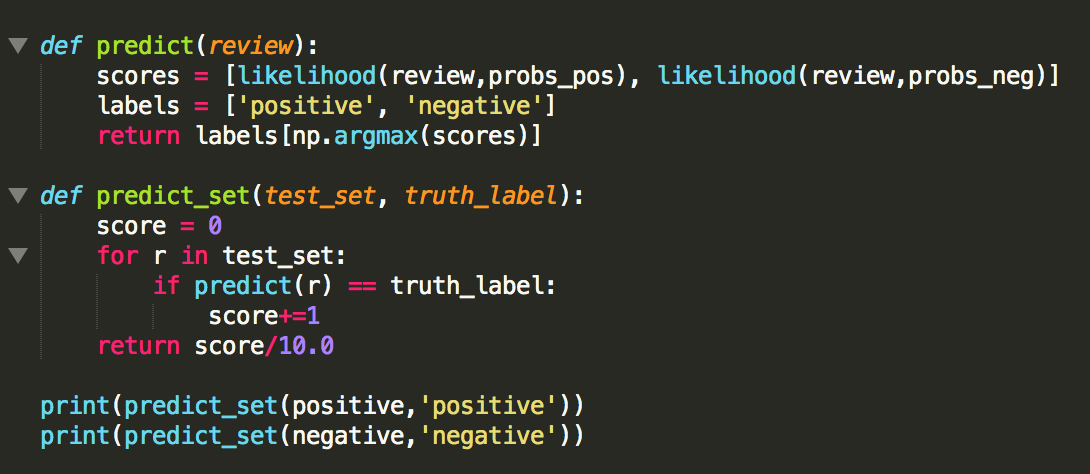
\includegraphics[width=0.7 \textwidth]{./figures/code_accuracy.png}
  \caption{Calculate the accuracy of each review prediction.}
\end{figure}

\subsection{10-fold cross-validation}

The 10-fold version of the code, increased the overall accuracy of the prediction. First, the code is parsed in a way to account for the 000 - 099, way of creating the folds for the positive and negative reviews. The code of the parsing is shown in Figure 23. Further, probabilities for each fold, are calculated in a similar matter to Figure 19, using numpy. Finally, the likelihood, predict, and predict\_set were modified in order to account for a fold parameter, to account for the current fold being used, this way the correct probabilities associated with that fold is used, that was the only change done to this functions, nevertheless the code is shown in Figure 24. 

To get the total accuracy, the individual accuracy per fold is stored in a list, this is then averaged and we get the total accuracy. The code that calculated this is shown in Figure 25. The results obtained by these code is shown in Figure 26. Finally, the confusion matrix for the 10-fold version is shown in Table 3. 

 \begin{figure}[htb]
  \centering
  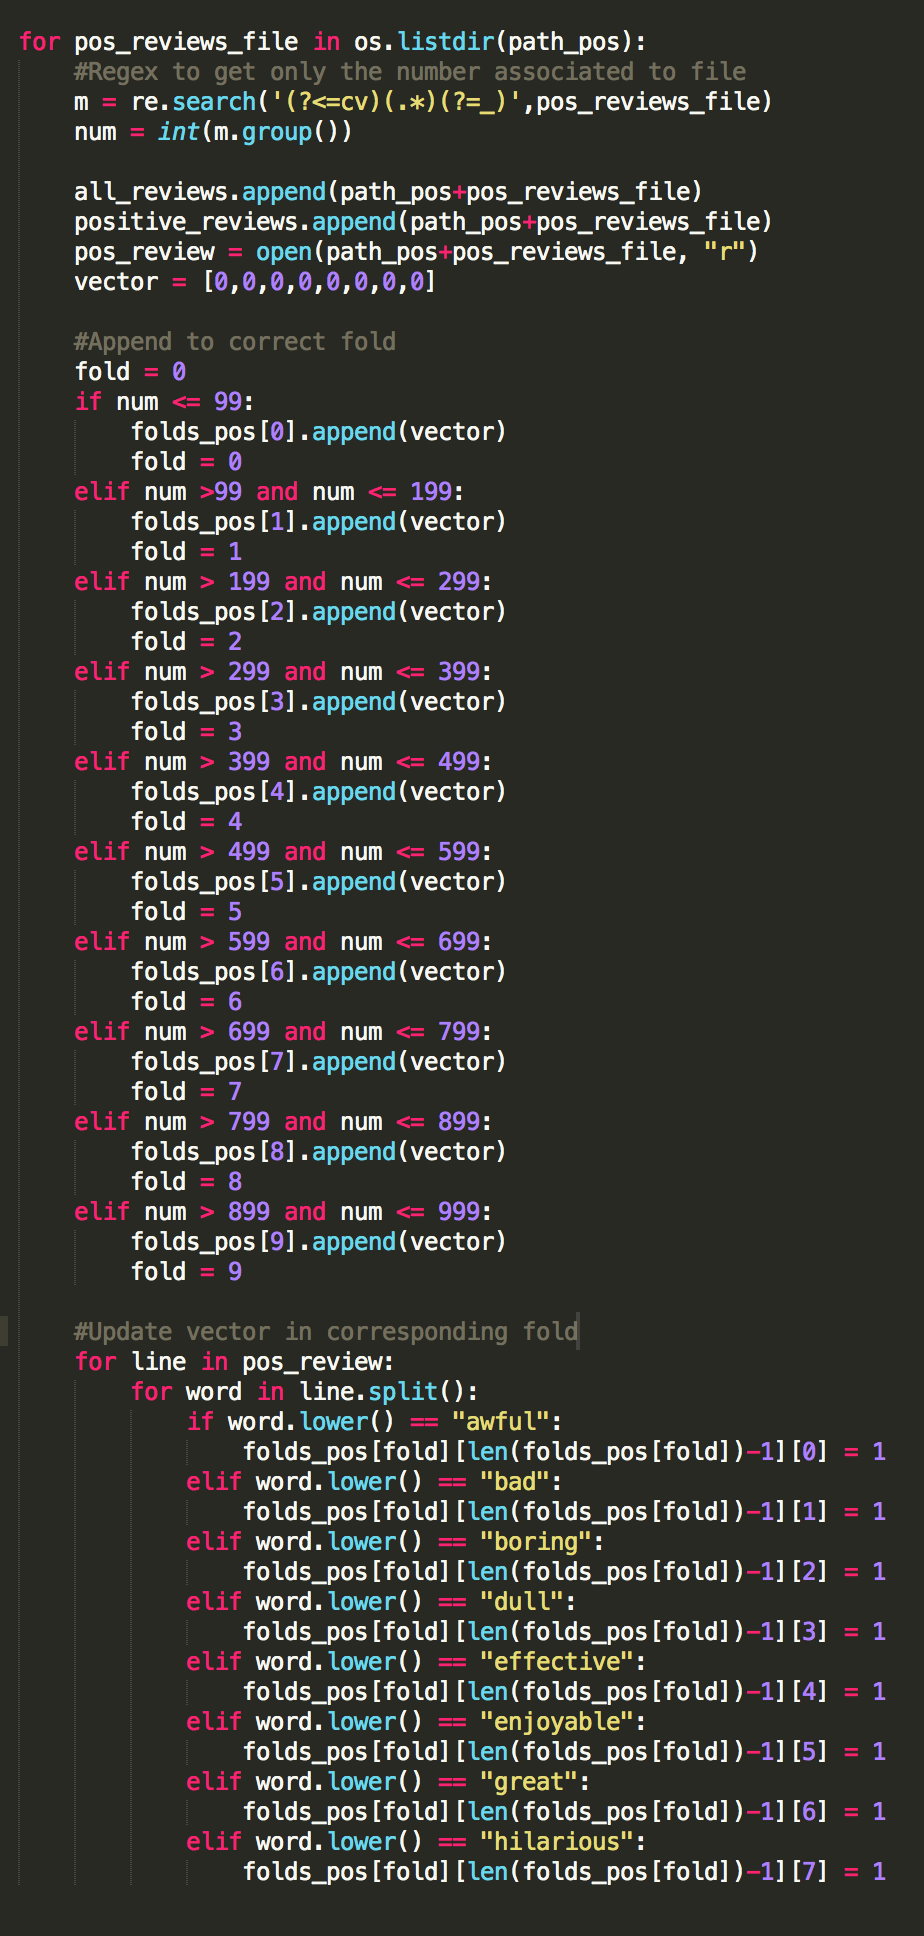
\includegraphics[width=0.6 \textwidth]{./figures/folds.png}
  \caption{Distributing vectors, into 10-folds.}
\end{figure}

\end{document}



%%% Local Variables:
%%% mode: latex
%%% TeX-master: t
%%% End:
